\section{实验及分析}
% 4-5 页

在本章节的实验环节,首先需要比较的是输入的数据集在参数规模上的横向差异,这对后续异常检测任务的效果差异的分析上具有作用;其次,由于本章所述方法是对数据集中图网络结构的变换,本文还将针对此方法输入和输出图网络的参数进行纵向对比,以初步分析所述方法在去除冗余边集和降低邻接矩阵稠密度上的效果。

在数字特征上反映出的优化效果仅反映在时间维度上,因而本文在接下来的对比实验中,采用了多种基于不同方法的模型以评估图网络生成算法在异常检测任务中的提升效果,从而评估算法在何种程度上保持和聚合数据集中原有拓扑特征;随后在案例分析中,本研究通过仿真的实验环境评估了两种方法在改善模型检测效果上的提升。

\subsection{数据集概述}

对于本章节提出的模型而言,它的性能不仅取决于是否能够在具有较强结构化拓扑特征的互联网数据集上取得良好的效果,还应当考虑其横向泛化特性,即是否能够适用于并不明显具有结构化拓扑特征的网络。先前章节提到了 DN42 是一类分布式网络,它相比由 IANA 管理的网络而言更具松散的结构而具有更少的层次性,适合用于本章节的实验部分。

在模型参数分析部分,由于未涉及到预设的异常参考值,本文采用了最近的来自两个分布式网络的路由数据,它们分别是采用了来自 RIPE RIS 的三个较近时间点的数据集和来自 DN42 的一个较近时间点的数据集,均采用 MRT 格式。相应的数据统计信息如表格 \ref{c3_data_input} 所示。

\begin{table}
    \caption{作为输入的路由数据集的统计信息}
    \begin{tabular}{lcccccccc}
        \toprule
        指标/数据集 & RIPE.2022.10 & RIPE.2022.11 & RIPE.2022.12 & DN42.2022.12 \\
        \midrule
        路由总数   & 10,068,040   & 10,072,615   & 10,165,549   & 82,664       \\
        前缀总数   & 103,162      & 104,265      & 104,523      & 716          \\
        \midrule
        节点总数   & 75,105       & 75,363       & 75,442       & 557          \\
        连边总数   & 2,228,343    & 2,230,203    & 2,246,004    & 2,756        \\
        \bottomrule
    \end{tabular}
    \label{c3_data_input}
\end{table}

在后续参数的使用上,对于基于相似度的构图方法的 k 值,本文从基于逻辑拓扑关系的构图结果中获取图网络的平均度数作为对应的值,具体的来讲,对于 RIPE 的几个数据集,它们的值为 4.35,对于 DN42 的数据集而言,它的值为 9.62,与基于 RIPE RIS 和 DN42 原始数据的估计是相近的。

% 数据量,表格 

\subsection{参数分析}

图网络参数是一个需要被首先考虑的问题,本文通过对上述三组来自 RIPE RIS 数据的输出连边数量及下降比例分析,总结出如表 \ref{c3_data_arg} 所示的结果。

从表 \ref{c3_data_arg} 中基于拓扑的模型的统计数据可以发现,该方法在对降低具有较多对等路由的网络连边数量具有较大的作用,这是该方法的原理所决定的,对于 RIPE 数据集而言,模型最大能够降低约 17\% 的无效连边数,其数量级约为 $10^6$ 左右,这在基于消息传递的多层图网络模型的嵌入效果和计算复杂度上会反映为较大的差异。

在 DN42 分布式网络数据集上,基于拓扑结构的构图算法并不能够取得与互联网数据集一致的边集优化效果,这一点可以从先前章节对 DN42 网络结构的概述中得到解释:具有实验性质的网络通常不具备较高的层次性,因而也存在较少的对等路由,对于此种广域网络系统上的路由异常检测需要更好的优化方案。

在基于相似度的图生成模型上,由于设定的参数 k 对边集大小具有控制作用,因而此处的数值对比意义不大,仅反映对应 k 值在路由数据集上的对应结果规模。在异常检测模型的实际运行中,需要兼顾计算效率和运算性能以确定最优的 k 值。

\begin{table}
    \caption{输入与输出的图网络参数对比}
    \begin{tabular}{llcccccccc}
        \toprule
        算法                     & 指标/数据集 & RIPE.2022.10 & RIPE.2022.11 & RIPE.2022.12 & DN42.2022.12 \\
        \midrule
        \multirow{2}{*}{基于拓扑}  & 输出连边 & 1,847,296    & 1,857,759    & 1,866,429    & 2,552        \\
                               & 下降比率   & 17.1\%       & 16.7\%       & 16.9\%       & 7.4\%        \\
        \midrule
        \multirow{2}{*}{基于相似度} & 输出连边 & 2,092,414    & 2,065,167    & 2,091,029    & 2,599        \\
                               & 下降比率   & 6.1\%        & 7.4\%        & 6.9\%        & 5.7\%        \\
        \bottomrule
    \end{tabular}
    \label{c3_data_arg}
\end{table}

\subsection{对比实验}

\subsubsection{分析指标}

% 跑一个模型,随机选取一系列路径,看对同一个新增路径数据的前后结果是否在同一个 rank 上。
为了检验数据集是否在拓扑特征上与处理前一致,本章节将已知的网络路由异常数据集提供给多个无监督的图嵌入模型,并分析在路由异常事件间的异常路由检出的准确度和 F1 值。具体地,本实验选择了 HOPE,DeepWalk,GraphSAGE 三种图网络嵌入的基线算法进行衡量,以标准化误差 0.5 作为异常阈值。

在数据集的选取上,对比实验选择了 RIPE RIS 于 2010、2017、2022 三个时间段上具有已知异常路由异常标记的数据集,使用异常发生前一天作为基准数据训练模型,并将路由异常开始后的流式路由更新输入到模型以获取路由异常检测的输出值作为对比。

\subsubsection{实验结果}

此实验采用了上述基线模型来评估图生成算法降低冗余和无效连边的性能,表 \ref{c3_s3tab} 报告了在不同模型下的异常检测结果,从中可以得到下列的发现:

\begin{enumerate}
    \item 相比于原始数据而言,基于拓扑和基于相似度的图构建方法与各基线模型的配合在大部分场景下能够取得异常检测结果的改善,这意味着本章所提出的模型达到了预期的效果。
    \item 基于拓扑的构图模型在总体上优于本实验中设定数值的基于相似度的构图模型,本研究将其归结于两种原因:
          \begin{enumerate}
              \item 其一是尽管基于相似度的构图方法能够通过对节点特征相似度的 topk 的方式降低原始数据在图上的稠密度,但它实质上并没有在根本上移除无效边集,因而在输出的图网络中引入了噪声。
              \item 其二是基于相似度的构图方法的效果完全依赖于 top-k 中确定的 k 值,而对于原始数据实际组成的图网络而言,节点的连边数量将会根据节点的重要程度产生不同的权重。
          \end{enumerate}
    \item 对于基于拓扑的图构建方法而言,总体上各异常检测模型在更具结构化、邻接节点和路由关系更加复杂的互联网路由数据集(RIPE 数据集)能够取得更好的效果,这是符合本研究的参数分析章节的预期的结果。
    \item 基于相似度的构图模型上在使用类似 DN42 的分布式网络数据集上存在性能不佳的问题,其中的一种可能原因是,管理松散、相互连接从而具有较少层次结构的分布式网络的节点之间的相似度距离会更加接近。
\end{enumerate}

\begin{table}
    \caption{对比实验结果}
    \begin{tabular}{lcccccccc}
        \toprule
                        & \multicolumn{2}{l}{RIPE.2010} & \multicolumn{2}{l}{RIPE.2017} & \multicolumn{2}{l}{RIPE.2022} & \multicolumn{2}{l}{DN42.2022}                                                                     \\ \cmidrule(lr){2-3} \cmidrule(lr){4-5} \cmidrule(lr){6-7} \cmidrule(lr){8-9}
        模型              & Acc.                          & F-1                           & Acc.                          & F-1                           & Acc.           & F-1            & Acc.           & F-1            \\ \midrule
        原始数据                                                                                                                                                                                                                \\
        \quad HOPE      & 0.712                         & 0.698                         & 0.708                         & 0.682                         & 0.709          & 0.688          & 0.692          & 0.671          \\
        \quad DeepWalk  & 0.768                         & 0.770                         & 0.754                         & 0.741                         & 0.750          & 0.757          & 0.751          & 0.755          \\
        \quad GraphSAGE & 0.793                         & 0.820                         & 0.815                         & 0.808                         & 0.784          & 0.814          & 0.807          & 0.801          \\ \midrule
        基于拓扑的构图模型                                                                                                                                                                                                           \\
        \quad HOPE      & 0.761                         & 0.754                         & 0.734                         & 0.721                         & 0.770          & 0.724          & 0.748          & 0.727          \\
        \quad DeepWalk  & 0.794                         & 0.784                         & 0.791                         & 0.786                         & 0.809          & 0.802          & 0.771          & 0.776          \\
        \quad GraphSAGE & \textbf{0.835}                & 0.824                         & \textbf{0.843}                & \textbf{0.821}                & \textbf{0.830} & \textbf{0.840} & \textbf{0.809} & \textbf{0.813} \\ \midrule
        基于相似度的构图模型                                                                                                                                                                                                          \\
        \quad HOPE      & 0.705                         & 0.703                         & 0.721                         & 0.715                         & 0.722          & 0.711          & 0.682          & 0.673
        \\
        \quad DeepWalk  & 0.780                         & 0.767                         & 0.778                         & 0.760                         & 0.762          & 0.752          & 0.759          & 0.770          \\
        \quad GraphSAGE & 0.823                         & \textbf{0.830}                & 0.820                         & 0.810                         & 0.812          & 0.826          & 0.801          & 0.807
        \\
        \bottomrule
    \end{tabular}
    \label{c3_s3tab}
\end{table}

\subsection{案例分析}

\subsubsection{实验方法}

为了确定模型性能的改善是由于图构建时采用的算法,本章基于 DN42 平台构建了仿真的测试环境,试图通过案例分析的方式确定算法的有效性。

如图 \ref{c3_case-flow} 所示,作为实验环境的初始化,节点 A(AS4242421331) 被接入到 DN42 网络中,并将其与 B(AS4201271332) 构成对等路由关系,其中 C(AS4242421331) 是 A 和 B 的共同 Transit 提供者,这是一个用于验证本章所述算法正确性的最小可操作场景。通过节点 A 向 DN42 的路由收集器发起路由反馈会话,并维持正常的网络路由一段时间,正常的路由表能够被 GRC 收集并生成数据集文件。

在随后的实验步骤中,节点 A 通过更长前缀的方式劫持节点 B 的路由,意图将通往该网络的流量劫持至节点 A 所控制的网络中。该行为将被网络自身及其各阶邻居通告给 GRC,随后 GRC 将以更新文件的形式将包含异常路由的路由表生成出来。

\begin{figure}[h]
    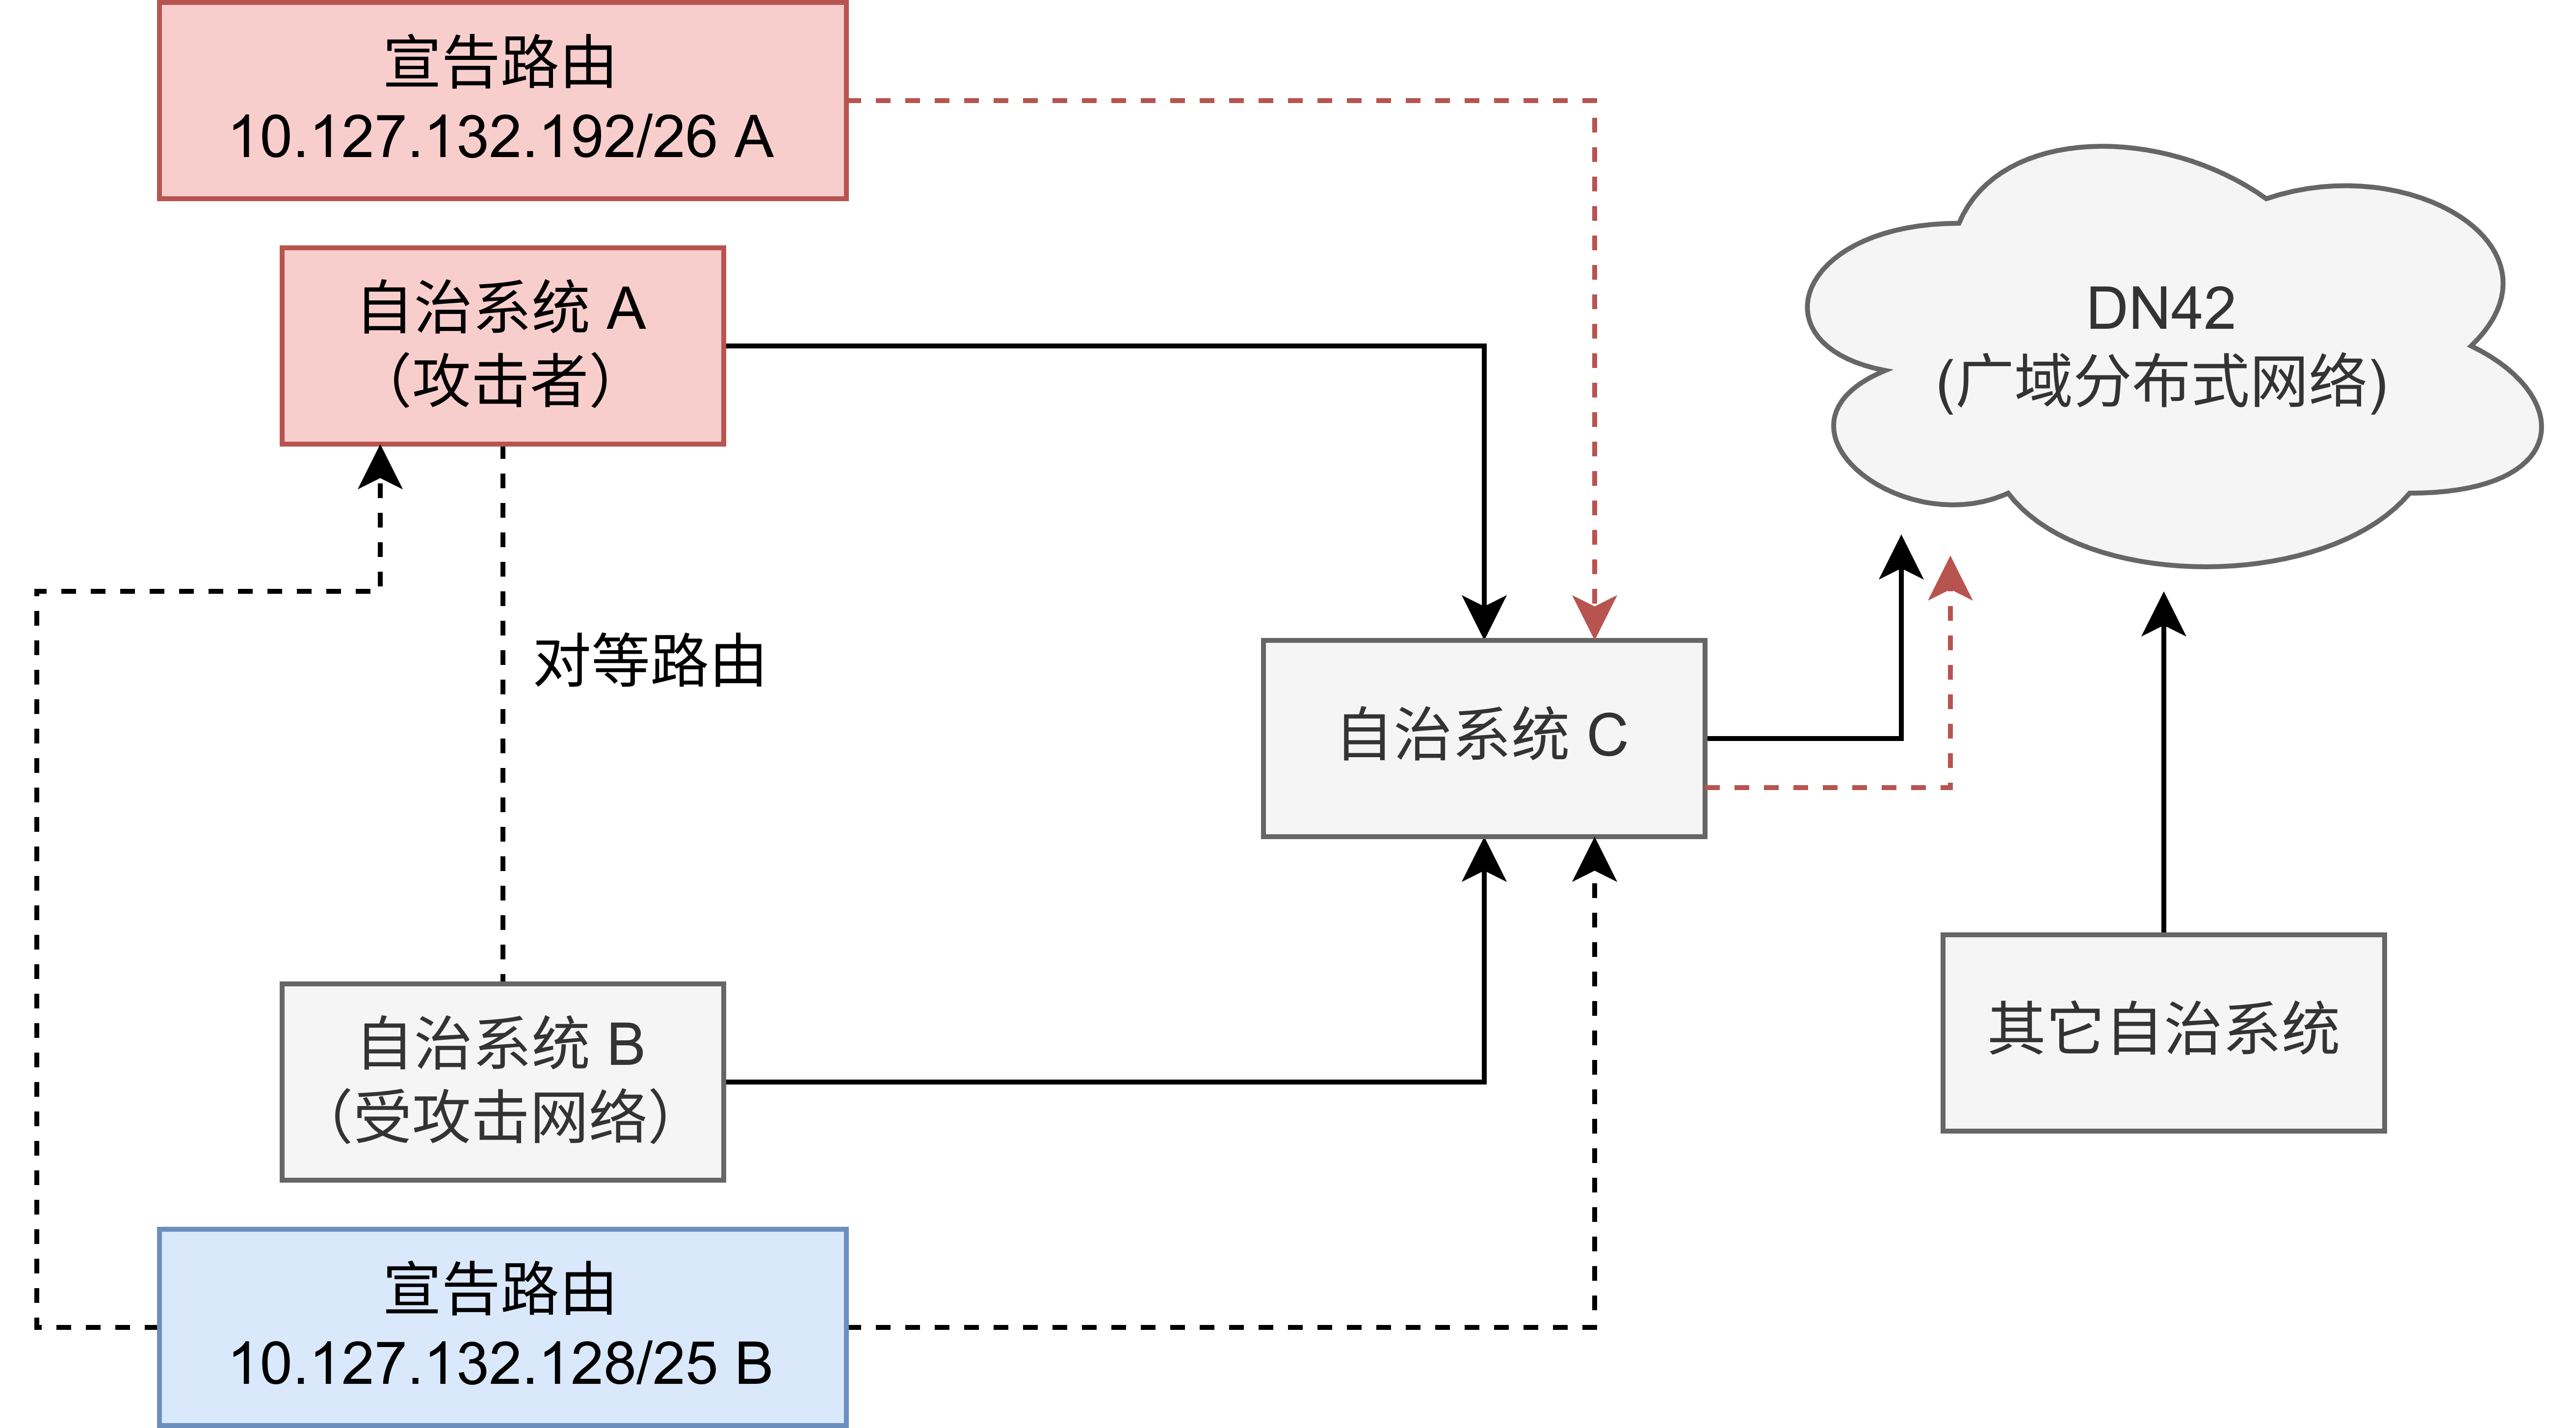
\includegraphics[width=0.7\linewidth]{chapter/c3_images/c3_case_flow.png}
    \caption{案例分析实验流程}
    \label{c3_case-flow}
\end{figure}

上述模型将以这两个文件作为输入,使用 GraphSAGE 算法模型进行嵌入并输出异常分数,从而判断本章所提出的算法对无效和冗余路由的去除效果,及对嵌入结果的影响。由于在此实验中,异常路由是已知的,因而可以从数据集中获取所有包含异常的路由样本,并将其送入模型进行异常检测。

基于对比实验的效果及在图构建算法设计上的规则,预期的结果是,使用原有数据集构成的路径的模型将在所有异常样本中取得相对更低的分数,而使用基于结构特征的构图方式的模型将在所有样本中取得相对更高的分数在,这是由于如图 \ref{c3_case-flow} 所示,在不去除自治系统 A 和自治系统 B 之间的对等路由的状况下,由原数据产生的图网络将包含 A、B 之间的连边,从而将 A、B 两个节点间的嵌入相似度拉近,进而影响到异常检测的分数。

\subsubsection{实验结果}

对于基于两种构图方式的所有异常路由样本的异常分数输出如图 \ref{c3_case-score} 所示。可见两种模型在异常样本的输出上与预期基本符合,与原始数据集相比在相同模型的分数输出上均具有提升。其中,基于结构特征的构图方式总体上对异常路由的预测效果提升最大(异常分数提升约 30\%),这反映出了基于结构特征的构图方式达到了相对而言更好的去除冗余路由的效果,而基于相似度的构图方式也相对于完全使用原始数据构图的方法在异常检测分数上提高了约 18\%,此结果展现出了,即使在不去除原始拓扑中的冗余路由的情况下,适当降低输入图网络的邻接矩阵稠密度同样能够改善模型的检测效果。

\begin{figure}[h]
    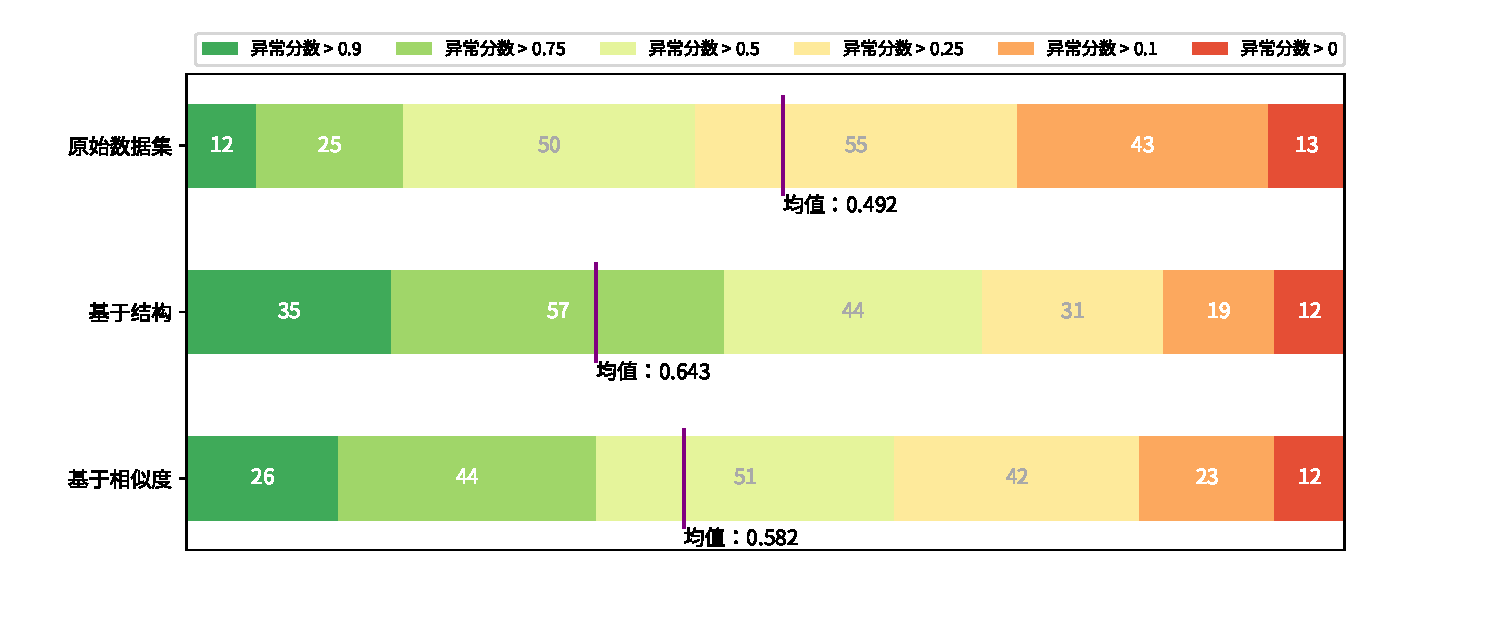
\includegraphics[width=\linewidth]{chapter/c3_images/c3_case-score.pdf}
    \caption{两种模型在异常路由样本下的输出分数}
    \label{c3_case-score}
\end{figure}